\documentclass[10pt,twocolumn,letterpaper]{article}
\usepackage[T1]{fontenc}
\usepackage[pagenumbers]{cvpr}
\usepackage{amsmath,amssymb,amsthm,booktabs,graphicx,microtype}
\definecolor{cvprblue}{rgb}{0.21,0.49,0.74}
\usepackage[pagebackref,breaklinks,colorlinks,allcolors=cvprblue]{hyperref}
\newtheorem{proposition}{Proposition}
\newcommand{\R}{\mathbb R}
\newcommand{\E}{\mathbb E}
\newcommand{\norm}[1]{\left\lVert#1\right\rVert}
\title{LatentAtlas: Few-Anchor Interfaces for Frozen Reward Transfer Across Autoencoders}
\author{Anonymous authors}
\begin{document}
\maketitle
\begin{abstract}
Latent reward models score image representations directly, but changing the autoencoder changes the coordinates they receive. We study whether a small set of same-image latent pairs can connect heterogeneous autoencoders to one existing reward. LatentAtlas learns a spatially shared interface to SD3.5 reference coordinates and reuses the complete frozen DiNa scoring path. Parameter fitting and checkpoint selection require neither reward queries nor preference labels. With 64 fitting and 64 validation images, a 39K-parameter interface preserves 94.64\% of native decisions for Cosmos and 94.72\% for FLUX on the same 28 development groups. Matched comparisons show higher decision agreement and lower reward-margin error than shared spatial affine regression in both sources. The interface also reduces margin error relative to two adapted SD-Latent-Interposer objectives, with additional agreement gains on FLUX. Correspondence controls and DC-AE experiments identify how the training pairs, target route, and image coverage affect functional transfer. A supporting model connects captured nonlinear signal and finite-anchor estimation error to selection regret for multiple frozen functions. These results establish a practical few-image interface for preserving a fixed latent reward and characterize the conditions under which coordinate adaptation delivers functional benefits.
\end{abstract}

\section{Introduction}
Latent diffusion systems represent images using learned autoencoders~\cite{rombach2022latent}. A reward operating directly on these representations can evaluate images without first constructing a pixel-space input to a separate visual encoder. DiNa develops this approach using a pretrained diffusion backbone and preference supervision~\cite{liu2026beyond}. Reusing such a reward across image generators creates an interface problem: changing the autoencoder changes channels, spatial resolution, coordinate scale, and feature statistics. Compatible tensor shapes alone do not establish compatible reward inputs.

A useful adaptation regime keeps the existing reward intact and learns only a small interface. For a new source autoencoder, a collection of images can be encoded in both source and reference coordinates. These same-image pairs provide supervision without requiring new preferences or queries to the reward during fitting. We call the paired images \emph{anchors}. The scientific question is how much frozen reward behavior this limited coordinate supervision preserves on other images.

\begin{figure*}[t]
\centering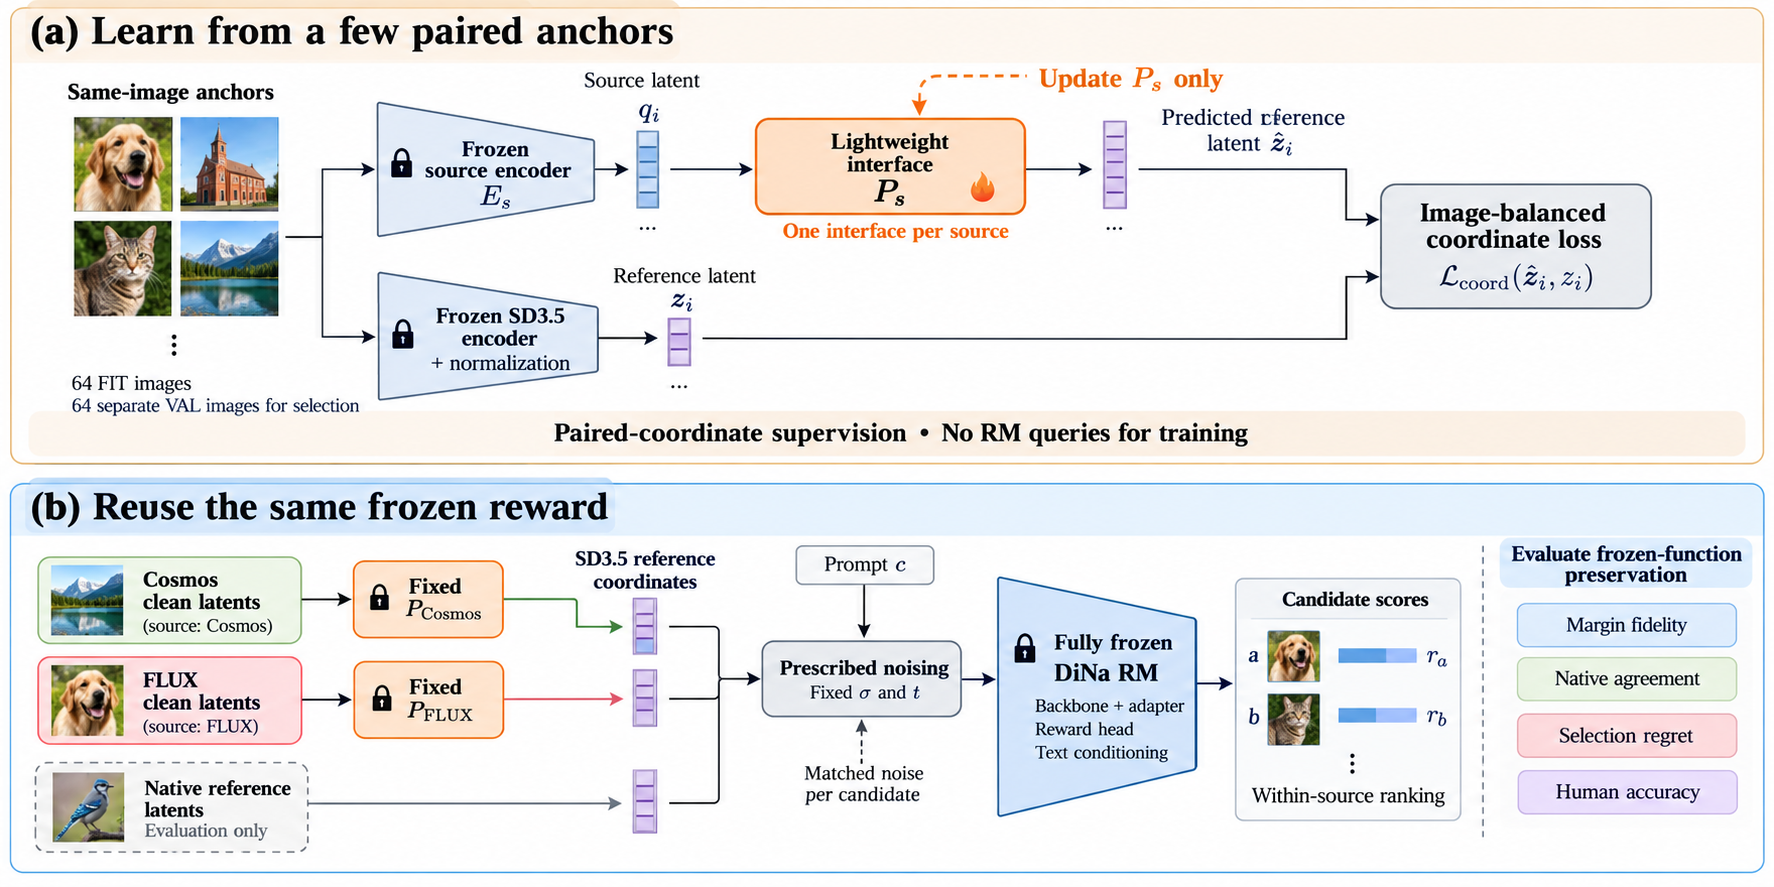
\includegraphics[width=\textwidth]{figures/clean/framework-user-20261020.png}
\caption{\textbf{Few-anchor adaptation and frozen reward reuse.} (a) Same-image encodings supervise a source-specific interface; the reported protocol uses 64 FIT images and 64 separate VAL images for coordinate-only selection. (b) Each fixed interface maps clean source latents to SD3.5 reference coordinates for the same frozen DiNa reward. Source branches are evaluated separately, with native latents as controls and matched noise per candidate occurrence. The prompt conditions DiNa; the noising operation acts on latent coordinates. Thumbnails illustrate the workflow.}
\label{fig:framework}
\end{figure*}

Representation matching provides a natural starting point. Model stitching learns interfaces between frozen components~\cite{csiszarik2021similarity,bansal2021revisiting}, and compact cross-VAE translators are available in practice~\cite{city96latentinterposer}. Preserving a preference reward adds a specific requirement: the mapped coordinates must retain score differences and candidate decisions. We evaluate this requirement under a few-image budget, comparing ordinary shared regression, lightweight nonlinear interfaces, and adapted cross-VAE translators.

LatentAtlas maps clean source latents to SD3.5 reference coordinates, then applies DiNa's original noising and prompt-conditioned scoring path (Fig.~\ref{fig:framework}). With 64 fitting and 64 validation images, the 39K-parameter REC interface reaches 94.64\% Cosmos and 94.72\% FLUX native decision agreement. Under matched adaptation budgets, its gains over shared spatial affine regression are 4.55 and 3.14 percentage points, respectively. Both sources also show lower margin MSE than either adapted Interposer objective, with additional agreement gains on FLUX.

Functional measurements reveal what the interface preserves. A historical Cosmos comparison improves margin error while leaving human-preference accuracy unchanged: 91.00\% of the net margin-error reduction occurs where the decision sign stays the same. In DC-AE, a larger bridge improves decisions without an established decrease in mean coordinate error. These complementary observations motivate evaluating coordinate reconstruction, score differences, and decisions together.

We make three contributions. First, we specify a few-anchor adaptation protocol that preserves the complete frozen reward and separates parameter-training, model-selection, and evaluation information. Second, we establish functional gains over strong shared regression and adapted cross-VAE translators on Cosmos and FLUX, and use correspondence controls and DC-AE studies to identify the roles of target construction and image coverage. Third, a complete-output supporting model gives a signal--estimation threshold under which one anchor-fitted interface improves multiple frozen selection functions over the affine class. The model supplies a conditional explanation for functional gains; the experiments measure those gains under the actual DiNa contract.

\section{Related Work}
\label{sec:related}
\paragraph{Functional representation matching.}
Model stitching asks whether a small interface can connect pretrained network components while preserving the target task~\cite{bansal2021revisiting,csiszarik2021similarity}. This functional criterion complements comparisons of representation geometry. Csisz\'{a}rik et al. distinguish direct matching of paired representations from fitting an interface through the downstream task loss, and evaluate least-squares, orthogonal, and reduced-rank mappings with the target network fixed~\cite{csiszarik2021similarity}. Their spatially shared affine operator motivates our simplest baseline. In foundation models, Mai et al. distinguish matching features at the stitch point, matching the target network's final features, and subsequent task-loss fitting~\cite{mai2026revisiting}. Local feature matching fits our coordinate-supervision budget; final-feature matching additionally reads and differentiates through the target suffix. We use an adapted local-matching MLP and shared spatial regressors to assess how much frozen reward behavior ordinary representation matching already recovers.

\paragraph{Corresponding anchors and latent translation.}
Relative representations encode a sample by its similarities to corresponding anchors, enabling communication through a common relative coordinate system~\cite{moschella2023relative}. Semantic Alignment instead estimates direct transformations between absolute representations from paired anchors, including linear, orthogonal, and affine maps~\cite{maiorca2023semantic}. Inverse Relative Projection reconstructs target-space coordinates from relative representations and target anchors~\cite{maiorca2024inverse}. These methods establish the usefulness of correspondences for exchanging pretrained modules. LatentAtlas uses same-image anchors as offline supervision for a spatial operator. At evaluation, that operator maps the current source tensor directly to the reference tensor; it does not retrieve the anchor set. The setting exposes a practical question about the number of independent images required to preserve a fixed preference function across heterogeneous autoencoders.

\paragraph{Cross-autoencoder interfaces.}
SD-Latent-Interposer provides convolutional translators between diffusion-autoencoder latents, including FLUX-to-SD3 conversion~\cite{city96latentinterposer}. Its released source uses paired-coordinate reconstruction, with configurable reverse and round-trip objectives. It is a direct precursor and a necessary comparator for cross-VAE adaptation. We focus on a specified low-data regime and evaluate preservation of a complete frozen preference reward, including score differences, native decisions, and human-preference accuracy. Comparing translators in this setting requires matching latent normalization, paired-image exposure, model selection, and optimization opportunity. Published weights with additional training data and architectures retrained on the same anchors represent distinct information budgets.

\paragraph{Latent rewards and reward-model reuse.}
DiNa learns a timestep-conditioned reward from diffusion representations and preference supervision, and supports noisy inputs and noise ensembling~\cite{liu2026beyond}. LatentAtlas reuses that learned preference function through its original input and scoring pathway. StitchVM transfers pixel-space rewards to noisy diffusion states by joining diffusion features to a reward suffix; its second training stage updates both the stitcher and that suffix using teacher-derived objectives~\cite{go2026stitchvm}. Our adaptation keeps the complete existing reward fixed and trains the interface from source/reference coordinates. These settings target different reuse contracts: learning a value model for noisy trajectories and preserving an existing latent reward after changing the input autoencoder. We study the latter using clean paired latents and the reward's prescribed noising procedure.

\paragraph{From alignment to functional risk.}
Representation-alignment theory relates regression mismatch to downstream risk under assumptions on the frozen readout~\cite{insulla2025alignment}. Such results motivate separating coordinate fit from functional preservation. Our analysis focuses on the competition between captured nonlinear signal and finite-anchor estimation error, using pair-selection regret as a functional endpoint. The empirical comparisons retain coordinate error, margin fidelity, native agreement, and human accuracy as separate measurements of the same fitted interface.

\section{Problem and Scoring Contract}
\label{sec:problem}
\paragraph{Paired observations.}
Let $E_s$ denote a frozen source encoder and $E_r$ the frozen reference encoder. Their definitions include image preprocessing, posterior sampling, coordinate normalization, and the spatial grid. Encoding the same image $x_i$ gives
\begin{equation}
 q_i=E_s(x_i),\qquad z_i=E_r(x_i),\qquad
 \mathcal A_s=\{(q_i,z_i)\}_{i=1}^{n}.
 \label{eq:anchors}
\end{equation}
The source-specific interface $P_{s,\theta}$ maps $q_i\in\R^{C_s\times H_s\times W_s}$ to the reference tensor shape. A new source is adapted with its own paired set and fitted parameters. The main experiments use $n=64$ fitting images and a disjoint set of 64 validation images. We count these as 128 images exposed during adaptation; spatial locations within an image share its identity.

\paragraph{Reference coordinates.}
The reference target is the SD3.5 posterior sample under a fixed image-identity seed, normalized once as $z=(q_r-0.0609)1.5305$. FLUX supplies its unshifted, unscaled, unpacked 16-channel posterior mode; Cosmos supplies its continuous 16-channel encoder output. The main two sources share the reference-resolution grid. DC-AE has 32 channels and a coarser grid, with a recorded fixed spatial conversion. Encoding mode and normalization are source-specific parts of the interface, rather than interchangeable conventions for tensors of the same shape.

\paragraph{Complete reward reuse.}
For prompt $c$, noise draw $\xi$, and scoring configuration $\tau$, the frozen score is
\begin{equation}
 R_\tau(z,c;\xi)=D_\phi((1-\sigma_\tau)z+\sigma_\tau\xi,c,t_\tau).
 \label{eq:reward}
\end{equation}
$D_\phi$ includes the diffusion backbone, its active adapter, the reward head, and text conditioning. Every component remains fixed. The evaluated configuration uses $\sigma_\tau=0.40029326$ and $t_\tau=400.29327$. Native evaluation supplies $z$; transferred evaluation supplies $P_{s,\theta}(q)$ to exactly the same path. The implementation preserves the recorded precision, quantization, and noise generation rules. Thus the interface predicts clean reference coordinates before the reward's own noising operation.

\paragraph{Training and selection information.}
Interface parameter fitting reads paired coordinates and FIT-derived statistics. Reward outputs, internal features, gradients, and preference labels are excluded from that objective. DiNa's pretrained preference knowledge is the fixed resource being reused~\cite{liu2026beyond}. The reported experiments also use coordinate-only checkpoint selection. We report selection information separately from parameter-training information: a procedure that uses reward evaluations to choose an interface incurs an additional, explicitly identified query budget. Evaluation data used for method development retain that status; confirmation data are reserved after method selection.

\section{Method: Few-Anchor Coordinate Interfaces}
\label{sec:method}
\subsection{A Spatially Shared Interface}
The interface learns a local transformation whose weights are shared across spatial positions. In the REC instantiation,
\begin{equation}
 P_{s,\theta}(q)=C_3\!\left(\rho\!\left(C_2\!\left(\rho(C_1(S_s(q)))\right)\right)\right),
 \label{eq:projector}
\end{equation}
where $S_s$ is the fixed source-grid conversion, $C_1,C_2,C_3$ are biased convolutions, and $\rho$ is SiLU. For FLUX and Cosmos, the kernels are $1\!\times\!1$, $3\!\times\!3$, and $1\!\times\!1$, with widths $16$--$64$--$64$--$16$ and 39,056 parameters. The spatial convolution uses zero padding. When resizing is required, the recorded implementation applies bilinear interpolation with \texttt{align\_corners=False} before the convolutions.

Spatial sharing concentrates the learning problem on a common local operator instead of assigning separate parameters to every image position. Nonlinear channel interactions allow it to represent correspondences beyond a shared affine map. Multiple locations supply training constraints, while the independent adaptation units remain images. At evaluation, the learned weights are fixed and the anchor images are no longer needed.

\subsection{Image-Balanced Coordinate Supervision}
Let $v_c$ be the reference channel variance computed from FIT data. REC minimizes
\begin{equation}
 \mathcal L(\theta)=\frac1n\sum_{i=1}^{n}\frac1{C_rH_iW_i}
 \sum_{c,h,w}\frac{(P_{s,\theta}(q_i)_{chw}-z_{i,chw})^2}{\max(v_c,10^{-6})}.
 \label{eq:loss}
\end{equation}
The channel weights balance errors across reference coordinates; the image average gives equal weight to differently sized images. These weights change the loss, not the stored latent coordinate system. Source standardization, when used by a baseline, is fitted separately on FIT and incorporated into its deployed mapping.

We fit REC with AdamW, an effective batch size of 32 images, and gradient-norm clipping at one. Full-image microbatches accommodate variable spatial grids. In the matched comparison, four learning rates and a common continuation rule determine the optimization opportunity for every neural family; separate coordinate validation selects each final checkpoint before reward evaluation (Section~\ref{sec:matched}). The supplement records the complete optimizer, schedule, precision, and historical fitting procedures.

\subsection{Mapping Classes and Comparison Budgets}
Shared affine regression tests how much transfer a linear spatial operator can recover. The matched baseline fits complete images with reflect-padded neighborhoods, an unpenalized intercept, and FIT-only source statistics. Coordinate validation selects among three neighborhood sizes and five regularization strengths. Historical pointwise and cropped spatial ridge fits provide additional diagnostics; their implementation and results appear in the supplement.

A2 is a 40,216-parameter spatial GELU interface with widths $16$--$144$--$120$--$16$, a $3\!\times\!3$ input convolution, and two $1\!\times\!1$ convolutions. It shares REC's variance-weighted objective. SD-Latent-Interposer~\cite{city96latentinterposer} supplies a larger cross-VAE architecture, evaluated with either that shared objective or its bidirectional reconstruction and round-trip objective. The historical pointwise MLP A1 adapts local feature matching~\cite{mai2026revisiting} with unweighted coordinate MSE. Together these comparators test the functional benefit of the fitted interface under explicit data and optimization budgets.

The matched comparison gives REC, A2, and both Interposer variants the same paired images, learning-rate trials, continuation rule, and selection information. Computational costs are recorded separately: the architectures have different parameter counts, and bidirectional training includes a reverse network.

\subsection{Functional Evaluation and Target Routes}
For a candidate pair $(a,b)$ under one prompt, define the native margin
\begin{equation}
 \Delta=R_\tau(z_a,c;\xi_a)-R_\tau(z_b,c;\xi_b),
\end{equation}
with $\widehat\Delta$ obtained by replacing each reference latent with its mapped counterpart. Native and mapped arms share the same noise for each candidate occurrence. Four fixed streams repeat the comparison. This pairing controls evaluation randomness without treating repeated streams as new images.

Coordinate error measures target reconstruction; margin MSE measures fidelity of score differences; native agreement measures preservation of the existing reward's decisions; and human accuracy compares decisions with annotated preferences. As a complementary selection endpoint, Native regret measures the native-score loss from choosing with the mapped score. It evaluates the value of a changed decision rather than counting all reversals equally. Its two-candidate expectation is
\begin{equation}
 \mathcal R(P)=\E\!\left[\max_{i\in\{a,b\}}S_i-S_{\hat\imath_P}\right],
 \quad \hat\imath_P=\arg\max_{i\in\{a,b\}}\widehat S_i,
 \label{eq:regret}
\end{equation}
where $S_i$ and $\widehat S_i$ are the coupled native and mapped scores. Tie rules, finite-stream aggregation, and group-level uncertainty are specified for each endpoint in the supplement. The empirical primary endpoints remain native agreement and margin MSE.

The main target is the reference encoding of the original image. A separate DC-AE experiment targets the reference encoding of the source-decoded reconstruction, using a larger Strong bridge. We retain its distinct teacher and scoring target when evaluating sample coverage. This separates learning an interface to the original reference from approximating a decode--re-encode route.

The complete procedure is to cache paired encodings, fit the chosen interface, apply its declared selection rule, and freeze it for coupled reward evaluation. Each result identifies the source, target route, image exposure, optimization budget, selection information, and scoring configuration. These choices connect the measured functional outcome to the actual adaptation procedure.

\section{Learning Signal and Frozen Decisions}
\label{sec:analysis}
A functional view separates the size of a coordinate error from its effect on a decision. For candidate $i$, write the score error as
$e_i=R_\tau(P_s(q_i),c;\xi_i)-R_\tau(z_i,c;\xi_i)$.
Then
\begin{equation}
 \widehat\Delta-\Delta=e_a-e_b,
 \label{eq:pairerror}
\end{equation}
and a nonzero native decision is preserved whenever
\begin{equation}
 |e_a-e_b|<|\Delta|.
 \label{eq:margin}
\end{equation}
Common score errors can cancel, and score changes within a margin leave the decision unchanged. Margin fidelity, decision agreement, and native regret therefore provide complementary measurements.

\paragraph{When does captured nonlinear signal pay off?}
A complete-output model makes the competition between useful signal and estimation error explicit. Let the source contain independent coordinates $X=(W,U_0,V_0,\ldots,U_r,V_r)$, where $W\sim N(0,I_k)$, each $U_\ell$ is a uniform sign, and each $V_\ell\sim N(0,1)$. Set $H=U_0V_0$ and $K=(U_1V_1,\ldots,U_rV_r)^\top$. The reference output and fixed functions are
\begin{equation}
 T(X)=BW+dH+GK,\qquad F_j(z)=a_j^\top z+b_j.
 \label{eq:supportmodel}
\end{equation}
Here $T$ contains the entire output read by each function. One interface fits all output coordinates by ordinary least squares on $n$ paired images, using the prespecified feature $\phi=(W,H)\in\R^p$, $p=k+1$. The fitted interface is $\widehat P(X)=\widehat C\phi(X)$, with coordinate OLS coefficient matrix $\widehat C$. The omitted interactions $GK$ supply estimation variance. The functions provide no training information.

Define $\theta_j=(B^\top a_j,a_j^\top d)$, $v_j=\|B^\top a_j\|^2$, $c_j=(a_j^\top d)^2$, and the fitted coefficient error $e_j^2=\|\widehat C^\top a_j-\theta_j\|^2$. Let $R_j$ be Native regret on a fresh iid candidate pair, with uniform selection on a predicted tie.
\begin{proposition}[Signal--estimation threshold]
\label{prop:signal}
In Eq.~\eqref{eq:supportmodel}, $A_0(X)=BW$ minimizes $R_j$ over all affine source interfaces, simultaneously for all $j$. Conditional on the fitted Anchor bank, if $e_j^2<c_j$, then every affine interface $A$ satisfies
\begin{equation}
 R_j(A)-R_j(\widehat P)\ge
 \frac{\sqrt{v_j+c_j-e_j^2}-\sqrt{v_j}}{\sqrt\pi}>0.
 \label{eq:signal}
\end{equation}
The strict error-radius threshold is sharp.
\end{proposition}
The proof uses the source's sign symmetry to establish the affine functional floor, then computes Gaussian pair-selection risk. For the coordinate OLS learner, $\E e_j^2=pq_j/(n-p-1)$, where $q_j=\|G^\top a_j\|^2$ and $n>p+1$. This gives a finite-image condition for one interface to improve all fixed functions; the supplement provides the full statement and proof.

The model predicts a benefit when captured functional signal exceeds its estimation cost. Its assumptions specify fixed features, Gaussian interactions, linear complete-output readouts, and independent deployment pairs. The empirical interfaces learn features jointly and are evaluated through nonlinear DiNa on grouped candidates; their measured functional outcomes establish the practical comparison. The supporting model guides a signal-versus-estimation interpretation, while the experiments directly test ordinary regression, nonlinear interfaces, target routes, and image coverage.

\section{Experiments}
\label{sec:experiments}
\subsection{Data, Controls, and Statistical Units}
The main comparison fits interfaces on 64 COCO images and selects checkpoints on 64 separate images. Evaluation uses 252 HPDv3 images in 28 connected candidate groups, forming 1,008 physical comparisons. Four noise streams produce 4,032 pair-stream observations. The data are image-disjoint from FIT/VAL, and the evaluation groups have been reused in the project's development. We therefore report them as a development evaluation throughout. Group bootstrap resampling preserves shared image and prompt dependencies; noise repetitions are not counted as independent images.

Native agreement excludes 33 native-tied pair-streams, leaving 3,999 observations, and awards half credit to an interface tie. Human accuracy uses all 4,032 observations, with ties incorrect. Each source comparison uses 50,000 shared group-bootstrap draws and its predeclared family of ten method pairs times two primary endpoints. Cosmos and FLUX share the same images, prompts, and native scores; they are two source-representation comparisons on one development set. Bonferroni-adjusted percentile intervals use quantiles 0.00125 and 0.99875. Historical comparisons retain their original nine- and six-endpoint families. The supplement provides the resampling and tie definitions.

\subsection{Matched Comparison with Strong Translators}
\label{sec:matched}
We compare REC, A2, shared spatial affine regression, and two adapted SD-Latent-Interposer objectives on the same FIT64/VAL64 images. Each neural family receives four 2,500-update learning-rate trials. A predeclared late-improvement rule triggers a common 2,500-update continuation at each family's coordinate-selected rate, totaling 100 validation checkpoints per family. Final checkpoints are fixed before reward evaluation. Affine selection covers three neighborhoods and five regularization strengths. Full training details appear in the supplement.

\begin{table}[t]
\centering\small
\begin{tabular}{lrrr}
\toprule
Interface & Native (\%) & Margin MSE & Human (\%)\\
\midrule
\multicolumn{4}{l}{\textit{Cosmos source}}\\
Spatial affine &90.09&.4708&72.12\\
Interposer-MSE &92.27&.2969&71.30\\
Interposer-cycle &92.67&.3491&71.43\\
REC &94.64&.1476&72.94\\
A2 &94.87&.1562&72.77\\
\midrule
\multicolumn{4}{l}{\textit{FLUX source}}\\
Spatial affine &91.59&.4721&72.89\\
Interposer-MSE &90.54&1.0728&69.72\\
Interposer-cycle &86.57&1.8445&69.32\\
REC &94.72&.2980&72.67\\
A2 &92.86&.3151&72.69\\
\bottomrule
\end{tabular}
\caption{Matched comparisons on the same 28 development groups. Within each source, neural families share paired images, search opportunities, and selection information. Cycle training uses additional reverse-network computation. Higher agreement and human accuracy, and lower margin MSE, are better.}
\label{tab:matched}
\end{table}

REC improves agreement over the selected affine baseline in Cosmos by 4.55 pp, adjusted interval $[1.16,8.98]$ pp, and in FLUX by 3.14 pp, $[.43,5.91]$ pp. Adjusted intervals for its margin-MSE differences are $[-.5408,-.1543]$ and $[-.3409,-.0335]$, respectively. On Cosmos, REC reduces margin MSE by 50.30\% and 57.73\% relative to Interposer-MSE and Interposer-cycle; their agreement differences remain unresolved. On FLUX, the corresponding margin reductions are 72.22\% and 83.84\%, and agreement gains are 4.19 pp, $[1.84,7.32]$ pp, and 8.15 pp, $[3.91,12.95]$ pp. All four absolute margin-difference intervals exclude zero. These source-specific comparisons establish functional gains for the small interface under the matched adaptation budget.

A2 improves margin MSE over all three baselines in each source. Its agreement gains are resolved against affine on Cosmos and cycle on FLUX. REC--A2 differences on both primary endpoints remain unresolved in both sources. Human-accuracy gains over affine remain unresolved; the FLUX gains over Interposer have positive descriptive intervals. Native fidelity and annotated preference accuracy therefore retain separate interpretations.

The Interposer comparison retrains its architecture under the present data and coordinate contract. The MSE variant uses the shared weighted objective; the cycle variant retains the released bidirectional loss and optimizer design, with full-image microbatches and BF16 computation. The historical A2 margin advantage over REC is absent from the resolved effects after matching optimization opportunities.

\subsection{Correct Correspondence Enables Transfer}
\label{sec:clean}
Historical controls isolate the information supplied by same-image pairing. With its original 1,000-update recipe, Cosmos REC reaches 93.41\% native agreement, compared with 59.68\% for the untrained interface and 59.43\% after permuting the fitting pairs. The permuted model is selected on true validation pairs, so the contrast tests fitting correspondence under the recorded selection procedure. One permutation and one initialization were evaluated. Historical FLUX REC reaches 91.69\% agreement. Full results and the original optimization budgets are retained in the supplement.

Human accuracies are 72.62\% for historical Cosmos REC and 72.79\% for FLUX REC, alongside 72.82\% for native DiNa. These observations show how much of the existing preference behavior survives coordinate adaptation; the matched comparisons above assess the additional value over strong alternative interfaces.

\subsection{What Ordinary and Stronger Mappings Explain}
The historical pointwise ridge reaches 90.91\% Cosmos agreement with 272 parameters, showing that simple shared regression captures much of the transfer. REC adds 2.50 percentage points (pp), simultaneous interval $[0.09,4.92]$ pp; its gain over the historical spatial ridge is 4.08 pp, $[1.57,7.78]$ pp. Both comparisons favor REC in margin MSE, while human-accuracy differences remain unresolved. The matched results in Table~\ref{tab:matched} extend this comparison to full-image affine fitting and common neural optimization opportunities.

Coordinate fit and reward fidelity can order interfaces differently. Relative to pointwise ridge, the historical spatial ridge reduces coordinate NMSE from 0.2978 to 0.1536, while margin MSE rises from 0.4604 to 0.5139. The between-ridge functional differences remain statistically unresolved; the marked coordinate improvement alone does not establish a reward improvement.

The historical A2 procedure reduces margin MSE from REC's 0.2338 to 0.1584, a 32.27\% improvement, and reaches 94.75\% native agreement. Human accuracy is exactly equal at the recorded precision. The original simultaneous intervals for REC minus A2 span zero for agreement, $[-3.20,0.013]$ pp, and human accuracy, $[-2.06,1.96]$ pp. This comparison includes A2's longer training and broader search; the matched comparison does not resolve an ordering between REC and A2.

\subsection{Where the Margin Improvement Occurs}


An aggregate accuracy equality can hide substantial changes. Across the 4,032 historical pair-stream observations, REC and A2 have the same ternary sign in 3,821 cases, reverse strict sign in 142, and change between a tie and a strict sign in 69. A2 repairs 90 human decisions and damages 90. The equality of human accuracy reflects this balance, rather than identical predictions.

The historical decomposition (visualized in the supplement) attributes 91.00\% of the net margin-MSE improvement to the unchanged-sign partition, 6.20\% to strict reversals, and 2.80\% to tie transitions. Contributions are signed: some individual rows worsen even within a partition whose aggregate improves. This decomposition explains the coexistence of better numerical fidelity and unchanged net human accuracy for these fitted models. It is consistent with the margin condition in Eq.~\eqref{eq:margin}, while leaving the source of individual coordinate errors open.

\subsection{DC-AE: Direct Mapping and Teacher Route}
\label{sec:dcae}
DC-AE provides a complementary source with 32-channel, coarser spatial latents. Applying the direct-to-reference recipe improves native agreement from 58.03\% for the untrained adapter and 58.64\% for the permuted control to 77.28\% for correct pairing. Human accuracy rises to 64.16\%, but remains 8.66 pp below native DiNa, with the recorded central 90\% interval $[-11.51,-5.88]$ pp. The direct recipe therefore recovers useful behavior while leaving a substantial functional gap.

To locate the gap, the round-trip route decodes the same source latent to an image and encodes that reconstruction with the reference autoencoder. Write
\begin{equation}
 T_0(x)=E_r(x),\qquad T_1(x)=E_r(D_s(E_s(x))).
 \label{eq:targets}
\end{equation}
The reward on $T_1$ is denoted $G$. This route reaches 97.47\% agreement with the original $T_0$ reward and 72.54\% human accuracy on the same development evaluation (Table~\ref{tab:dcae}). It exhibits a realizable higher-fidelity path from the source code using substantial pretrained decoding and encoding computation. The direct and round-trip routes use different pretrained computation and interface classes, making the latter a functional reference for the tested direct mapping.

\begin{table}[t]
\centering\small
\begin{tabular}{lrr}
\toprule
DC-AE route on DEV28&Native agr. (\%)&Human (\%)\\
\midrule
Untrained direct REC&58.03&43.06\\
Permuted direct REC&58.64&48.69\\
Correct direct REC $\to T_0$&77.28&64.16\\
Decode--encode $\to T_1$ ($G$)&97.47&72.54\\
Native $T_0$&100.00&72.82\\
\bottomrule
\end{tabular}
\caption{Teacher-route localization, with the original reference reward as the agreement target. The round-trip route uses the source decoder and reference encoder in addition to the frozen reward.}
\label{tab:dcae}
\end{table}

A separate mapping-class comparison trains small and Strong bridges toward $T_1$ for 2,000 updates. Strong improves human accuracy by 3.57 pp and agreement with the original-reference reward on $T_0$ by 6.16 pp over the small bridge; adjusted interval lower bounds are 1.54 and 3.50 pp. The small bridge has mean $T_1$ coordinate NMSE 0.3092 and Strong has 0.3104, with an unresolved difference. This supplies the converse of the ridge observation: improved functional decisions can occur without an established improvement in aggregate coordinate error. The scalar coordinate metric does not determine the downstream ordering.

\subsection{Increasing Anchor Coverage at Fixed Updates}
\label{sec:anchors}
The DC-AE Strong bridge also supports an actual fitting-budget comparison. We retain the $T_1/G$ teacher, 889,424-parameter architecture, initialization seed, effective batch size 32, and 2,000 updates. FIT256 contains FIT64 plus 192 images from the same COCO pool, while VAL64 remains fixed. Both arms start from step zero and process 64,000 image presentations; the wider support reduces the average reuse of each fitting image. The experiment fixes updates and total presentations while varying unique-image coverage and per-image reuse.

Evaluation uses 504 images in 56 groups, forming 2,016 physical pairs. These groups are disjoint from the earlier adapter development groups, but their parent pool was used for source qualification. They provide a separate adapter evaluation, with that prior scientific consumption retained in its interpretation.

\begin{table}[t]
\centering\small
\begin{tabular}{lrr}
\toprule
Endpoint on 56 groups & FIT64 & FIT256\\
\midrule
$T_1$ coordinate NMSE$\downarrow$&0.2963&0.2100\\
Agreement with $G$ (\%)$\uparrow$&85.88&88.69\\
Human accuracy (\%)$\uparrow$&68.54&69.95\\
\bottomrule
\end{tabular}
\caption{DC-AE Strong: larger paired-image support at fixed updates. Both arms use the same 64 VAL images. This is a round-trip-target experiment; its agreement target is $G$, distinct from the original-reference target in Tables~\ref{tab:matched} and~\ref{tab:dcae}.}
\label{tab:anchors}
\end{table}

All three endpoints improve (Table~\ref{tab:anchors}). Coordinate NMSE falls by 29.11\%, with a three-endpoint-adjusted interval of $[26.56,31.78]\%$. Agreement with $G$ increases by 2.82 pp, interval $[1.34,4.28]$ pp; human accuracy increases by 1.41 pp, interval $[0.46,2.41]$ pp. At the same time, error on the shared original FIT64 increases from 0.1806 to 0.2107. The wider fitting support improves performance on the evaluated non-fitting images despite worse fit to that original subset. This nested support expansion improves the evaluated endpoints with the teacher route and initialization held fixed.

\section{Discussion and Limitations}
The central practical result is that a small, spatially shared interface can preserve a frozen latent reward from a few paired images. Ordinary regression already recovers much of the behavior; the matched comparisons establish REC's additional agreement and margin fidelity over affine regression in both sources, as well as margin gains over both adapted Interposers and agreement gains over them on FLUX. The comparison matches data, selection information, and optimization opportunity. Its architectural attribution remains broader than a specific activation or nonlinear component, and the computation differs across families.

The diagnostic experiments explain why functional evaluation is essential. Coordinate recovery, margin fidelity, native decisions, and annotated preferences measure different consequences of the same mapping. Historical margin improvements concentrate in already-preserved decisions, while DC-AE reveals gains from changing the mapping class and increasing image coverage. The supporting model formalizes a signal--estimation tradeoff for fixed features and readouts; applying that mechanism to learned interfaces and nonlinear DiNa requires further evidence.

The principal empirical boundary is the evaluation data's development history. Cosmos and FLUX are two source representations of the same 28 groups; the separate DC-AE groups have prior source-qualification use. An untouched post-selection confirmation set is needed for confirmatory performance claims. Source families, initialization draws, and fitting budgets remain limited, and the $T_1/G$ coverage study lacks a matched ridge baseline. The demonstrated capability is clean-image, within-source reward reuse. Native noisy-state transfer, mixed-source score calibration, and end-to-end compute savings remain separate deployment questions.

\section{Conclusion}
LatentAtlas connects heterogeneous autoencoders to one completely frozen latent reward using same-image coordinate anchors. With 64 fitting and 64 validation images, a 39K-parameter interface preserves about 94.6--94.7\% of native decisions on the evaluated Cosmos and FLUX development representations. Matched comparisons establish functional gains over shared affine regression and adapted cross-VAE translators, with endpoint-specific differences between sources. Correspondence controls, decision-level analysis, and DC-AE studies show how target construction and image coverage shape those gains. Together, the protocol and evidence make few-anchor reward reuse a concrete, measurable capability and identify the conditions to test when extending it to new generators.

{\small\bibliographystyle{ieeenat_fullname}\bibliography{references}}
\end{document}
